\documentclass{article}

% if you need to pass options to natbib, use, e.g.:
% \PassOptionsToPackage{numbers, compress}{natbib}
% before loading nips_2018

% ready for submission
\usepackage[final]{nips_2018}

% to compile a preprint version, e.g., for submission to arXiv, add
% add the [preprint] option:
% \usepackage[preprint]{nips_2018}

% to compile a camera-ready version, add the [final] option, e.g.:
% \usepackage[final]{nips_2018}

% to avoid loading the natbib package, add option nonatbib:
% \usepackage[nonatbib]{nips_2018}

\usepackage[utf8]{inputenc} % allow utf-8 input
\usepackage[T1]{fontenc}    % use 8-bit T1 fonts
\usepackage{hyperref}       % hyperlinks
\usepackage{url}            % simple URL typesetting
\usepackage{booktabs}       % professional-quality tables
\usepackage{amsfonts}       % blackboard math symbols
\usepackage{nicefrac}       % compact symbols for 1/2, etc.
\usepackage{microtype}      % microtypography
\usepackage[vlined,ruled,commentsnumbered,linesnumbered]{algorithm2e}
\usepackage[fleqn]{amsmath}
\usepackage{listings}
\usepackage{graphicx}
\usepackage{subfigure}
\usepackage{color,xcolor}
% \usepackage{fontspec}
% \setmainfont{Times New Roman}

\title{CS420 Project Report}

% The \author macro works with any number of authors. There are two
% commands used to separate the names and addresses of multiple
% authors: \And and \AND.
%
% Using \And between authors leaves it to LaTeX to determine where to
% break the lines. Using \AND forces a line break at that point. So,
% if LaTeX puts 3 of 4 authors names on the first line, and the last
% on the second line, try using \AND instead of \And before the third
% author name.

\author{
  Ruiheng Chang \\
  515021910459\\
  Department of Computer Science\\
  Shanghai Jiao Tong University\\
  \texttt{crh19970307@sjtu.edu.cn}
  \And
  Weichao Mao \\
  515021910559\\
  Department of Computer Science\\
  Shanghai Jiao Tong University\\
  \texttt{maoweichao@sjtu.edu.cn}
  %% \AND
  %% Coauthor \\
  %% Affiliation \\
  %% Address \\
  %% \texttt{email} \\
  %% \And
  %% Coauthor \\
  %% Affiliation \\
  %% Address \\
  %% \texttt{email} \\
  %% \And
  %% Coauthor \\
  %% Affiliation \\
  %% Address \\
  %% \texttt{email} \\
}

\begin{document}
% \nipsfinalcopy is no longer used

\maketitle

\section{Traditional Models}
In this section, we first preprocess the images on the pixel level to remove the disturbances. We then perform traditional classification models, such as KNN and SVM, on the processed images. We further compare the performance of the traditional models with and without the preprocessing procedure. Finally, we employ ensemble methods and try to obtain better predictive performance.

\subsection{Pixel-Level Image Preprocessing}
We can easily see the data set given to us is generated by adding some minor disturbances to the standard MNIST data set. These disturbances include spatial shifting of the main digit, and small random pepper noise which presents itself as sparsely occurring white pixels. 

Before applying traditional machine learning algorithms on the disturbed MNIST data set, we first perform pixel-level preprocessing on the images, aiming to reverse the disturbances and reconstruct the original images. In the following, we will demonstrate our preprocessing procedure step by step.

\subsubsection{Timeline Overview}
The preprocessing steps are summarized in Figure~\ref{fig:preoverview}. Figure\ref{subfig:original} shows one original image from the given data set. As we can see, there is a patch of white noise on the right side, and the digit is located in the lower half of the image. Our first step in the preprocessing removes the white noise on the right, and the denoised result is shown in Figure\ref{subfig:denoised}. In the second step, we crop out the minimum rectanglar area that covers the digit pixels, and Figure~\ref{subfig:cropped} shows the cropped digit. Finally, Figure~\ref{subfig:centered} shows the centered image after we add equal padding to the digit. 

\begin{figure}[!htb]
	\centering
	\subfigure[Original]{
	\label{subfig:original}
	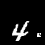
\includegraphics[width=.2\textwidth]{fig//3_original.png}
}
	\subfigure[Denoised]{
	\label{subfig:denoised}
	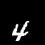
\includegraphics[width=.2\textwidth]{fig//3_denoised.png}	
}
\subfigure[Cropped]{
	\label{subfig:cropped}
	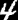
\includegraphics[width=.18\textwidth]{fig//3_cropped.png}	
}
\subfigure[Centered]{
\label{subfig:centered}

\includegraphics[width=.2\textwidth]{fig//3_centered.png}	
}
\caption{Preprocessing timeline overview.}
\label{fig:preoverview}
\end{figure}

\subsubsection{Step 1: Denoising}
The first step concerns searching and removing the white pepper noise in the image. In this step, we regard any white pixel block with no more than 20 connected pixels as the noise area. The intuition is, the pixels of digits 0 to 9 are all connected blocks, and since the digit is the main part in the image, it must contain a large area of pixels (more than 20 pixels). 

We utilize the simple Depth First Search (DFS) algorithm to search for the connected blocks. We enumerate each of the pixels in the image starting from the upper-left corner. If the current pixel is a white pixel, we will further check its 8 neighboring pixels and if there exist white pixels among its neighbors, we connect them into a single block. Figure\ref{fig:DFS} demonstrates the detailed process of this step. Suppose the original binary image is shown in Figure\ref{subfig:binary}. For a white pixel we are visiting (colored in blue in Figure\ref{subfig:neighbors}), we need to further check its 8 neighbors. Since we find two more white pixels among its neighbors (colored in yellow in Figure\ref{subfig:neighbors}), we connect the three pixels into a single block, and repeat the same procedure on the two neighboring white pixels. Finally, we will find the whole white connected block. 

\begin{figure}[!htb]
	\centering
	\subfigure[Original image]{
		\label{subfig:binary}
		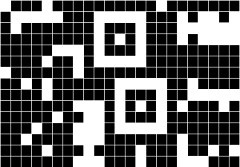
\includegraphics[width=.45\textwidth]{fig//DFS1}
	}
	\hspace{.2in}
	\subfigure[Neighbors]{
		\label{subfig:neighbors}
		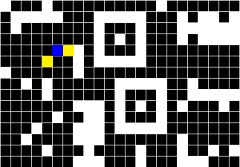
\includegraphics[width=.45\textwidth]{fig//DFS2}	
	}
	\caption{White block searching.}
	\label{fig:DFS}
\end{figure}

Once we have found the noise area (i.e., the white connected blocks with area no more than 20 pixels), the denoising process is easy to implement. We only need to employ the Flood Fill algorithm on the noise areas, and color the white pixels into black. A different statement of the same process is to perform a second DFS on the noise pixels, and color every white pixel we visit into black. 

\subsubsection{Step 2: Cropping}

So far, we have safely removed the white pepper noises from the images, but we still cannot feed the current digit into the traditional models directly. The problem is, the digits are not centered in the image, and although some models like convolutional neural networks are not sensitive to shifting, these misaligned digits can rule out many traditional models like KNN. To guarantee a reasonable performance of the traditional models, we further need to center the digital pixels right in the middle of the image.

This second step is relatively easy. We only need to find the boundaries of the digit and crop it out. As illustrated in Figure\ref{fig:crop}, we can enumerate to find the upper-most, left-most, right-most and lower-most pixels in the denoised image, and use these pixels as boundaries (denoted by yellow lines in Figure\ref{subfig:bar}) to crop out the digital area.

\begin{figure}[!htb]
	\centering
	\subfigure[Boundaries]{
		\label{subfig:bar}
		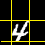
\includegraphics[width=.2\textwidth]{fig//3_denoised_bar}	
	}
\hspace{.2in}
\subfigure[Cropped digit]{
	\label{subfig:cropped2}
	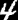
\includegraphics[width=.18\textwidth]{fig//3_cropped.png}	
}
	\caption{Cropping out the digit.}
	\label{fig:crop}
\end{figure}

\subsubsection{Step 3: Centering}
Finally, we will center the digital area right in the middle of the image. We want to keep the size of the image ($45\times 45$) unchanged before and after the preprocessing procedure so that we can simply feed the new data set into our other models. Since the size of the cropped image can be a little smaller than the original image, we add equal padding to the left, right, up and down side of the digit to make its size equal to the original one. The equal padding also guarantees the digit will always be centered in the image, so that the misalignment of digits is not a problem anymore. The OpenCV library provides a function \textit{copyMakeBorder} that implements this operation. Therefore, we only need to calculate the padding length and then safely rely on OpenCV to do the padding job. 


\begin{figure}[!htb]
	\centering
	\subfigure{
		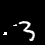
\includegraphics[width=.2\textwidth]{fig//9_original.png}
	}
	\subfigure{
		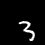
\includegraphics[width=.2\textwidth]{fig//9_denoised.png}	
	}
	\subfigure{
		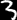
\includegraphics[width=.17\textwidth]{fig//9_cropped.png}	
	}
	\subfigure{
		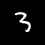
\includegraphics[width=.2\textwidth]{fig//9_centered.png}	
	}

\subfigure{
	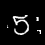
\includegraphics[width=.2\textwidth]{fig//19_original.png}
}
\subfigure{
	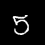
\includegraphics[width=.2\textwidth]{fig//19_denoised.png}	
}
\subfigure{
	
\includegraphics[width=.17\textwidth]{fig//19_cropped.png}	
}
\subfigure{
	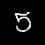
\includegraphics[width=.2\textwidth]{fig//19_centered.png}	
}

\subfigure{
	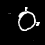
\includegraphics[width=.2\textwidth]{fig//30_original.png}
}
\subfigure{
	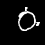
\includegraphics[width=.2\textwidth]{fig//30_denoised.png}	
}
\subfigure{
	
\includegraphics[width=.183\textwidth]{fig//30_cropped.png}	
}
\subfigure{
	
\includegraphics[width=.2\textwidth]{fig//30_centered.png}	
}

	\caption{More examples of preprocessing, including failure cases.}\label{fig:moreexample}
\end{figure}

So far, we have finished our preprocessing steps, and the images are ready to be feed into the traditional models. Figure\ref{fig:moreexample} lists more examples of our preprocessing results. Please be aware there also exist some failure cases. For the digit 0 in the third row of Figure\ref{fig:moreexample}, since the pepper noise area is directly connected with the digital area, our denoising step regards the noise as part of the digit and fails to remove it from the image. Although some further morphological image processing techniques can help remove these noises, we consider our current results as already satisfactory, because the failure cases are really rare among the data samples. For more detailed explanations of our preprocessing steps, please refer to the comments in our code in file \texttt{preprocessing.py}.

\subsection{K-Nearest Neighbors}
In this part, we utilize the simplest classifier, the K-Nearest Neighbors algorithm, or KNN, on the given data set as well as our processed data set. KNN is a non-parametric model. An test data sample is classified by a majority vote of its neighbors. More specifically, the data point is assigned to the class that is most common among its $k$ nearest neighbors. 

The reason we choose this algorithm is that we are clear KNN is very sensible to the spatial shifting of the digits in the image. By comparing the KNN output on the given data set with its output on our processed data set, we can easily check whether our preprocessing step is helpful or not, and to what extent the preprocessing helps improve the performance. 

Before we perform KNN on the data sets, we first refer to Principal Component Analysis, or PCA, to reduce the dimensionality of the data sets. We will not dig into the theoretic details of PCA (and KNN) in this report since they are all well covered in the course lectures. All we need to care about is that the specific PCA ratio will have a significant influence on the performance of our models. The scikit-learn library provides the PCA and KNeighborsClassifier classes so that we can safely rely on these modules to achieve our goal. For more detailed programming implementation of this part, please refer to our codes in files \texttt{KNN\_without\_preprocessing.py} and \texttt{KNN.py}.

Throughout our experiments, we use the simple hold-out validation, and randomly select 30\% of the training samples as our validation set. We also fix the distance metric as L2 distance. We test the KNN performance of different setting of parameters on the validation set, and select the parameter values with highest accuracy to feed into the model on the test set.

\subsubsection{Influence of PCA Ratio}
In this part, we test the influence of PCA ratio on KNN. We enumerate the PCA ratio value from $0.3$ to $1.0$, and for each PCA ratio value, we enumerate the value of $k$ on the validation set to find the optimal value under the current PCA ratio. Since this nested iteration process is relatively time consuming, we only use 10000 training samples and 3000 testing samples in this part. The performance of KNN on the given data set and our processed data set under different PCA ratio values is shown in Figure~\ref{fig:KNN_PCA}. From Homework 3 we know that the size of training samples will indeed influence the performance of our model, and the performance shown in Figure\ref{fig:KNN_PCA} is definitely worse than it should be. Still, we believe the trend of the performance is the same even under smaller number of training samples. The values of $k$ for KNN are separately optimized for the two validation set under each specific value of PCA ratio. 


\begin{figure}[!htb]
	\centering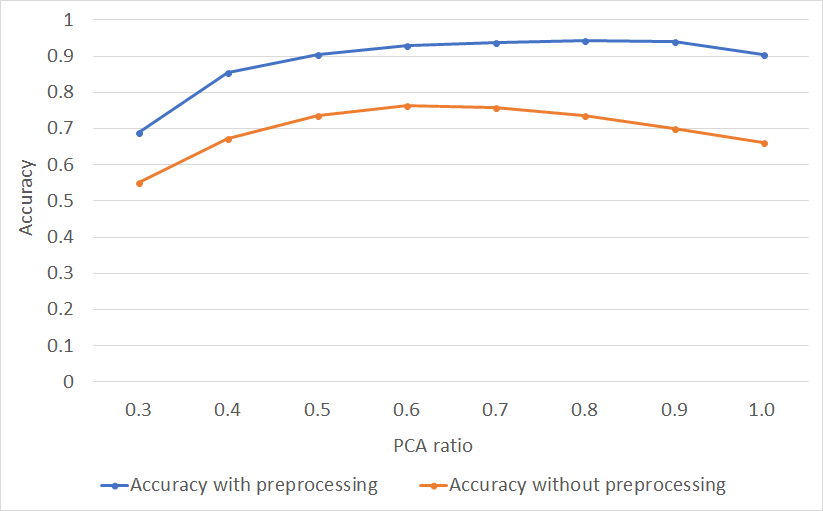
\includegraphics[width=.8\textwidth]{fig//KNN_PCA}
	\caption{KNN performance under different PCA ratios.}\label{fig:KNN_PCA}
\end{figure}

As we can see, for KNN both with and without preprocessing, the accuracy first increases with PCA ratio and then decreases. The highest accuracy of KNN with preprocessing is achieved at PCA ratio equals 0.8, and for KNN without preprocessing the optimal PCA ratio is 0.6. This indicates that the high dimensional image data samples indeed contain some level of redundancy, and dimensionality reduction can help KNN improve performance. Another fact to notice is that KNN with preprocessing always outperforms its counterpart without preprocessing. This indicates our preprocessing procedure can indeed help traditional models avoid spatial shifting issues.

\subsubsection{Influence of K}
In this part, we test the influence of the $k$ value for KNN. The value of $k$ really depends on the data set, and is crucial to the performance of the model.

\begin{figure}[!htb]
	\centering
	\subfigure[K=1.]{
		\label{subfig:1NN}
		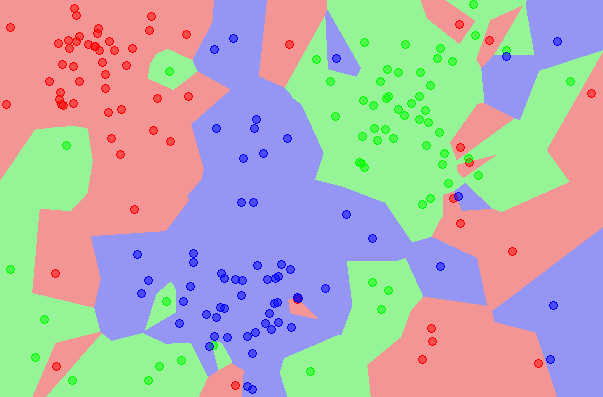
\includegraphics[width=.4\textwidth]{fig//1NN.png}}
	\hspace{.2in}
	\subfigure[K=5.]{
		\label{subfig:5NN}
		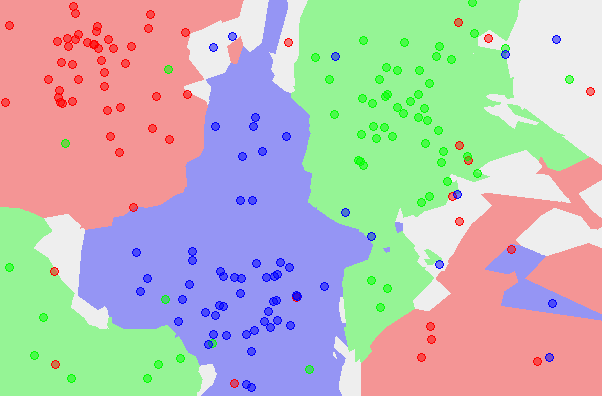
\includegraphics[width=.4\textwidth]{fig//5NN.png}}
	\caption{KNN performance under different values of $k$.}\label{fig:KNN}
\end{figure}

Generally speaking, a larger $k$ can make the model more resistant towards noises and outliers, but may also renders the classification boundary more blurred. Figure\ref{fig:KNN} demonstrates the performance under different values of $k$ on the same data set. As we can see, the boundaries become more smoothed as $k$ increases, and the model is getting more robust against outliers. There are some heuristic algorithms dedicated to finding the optimal value of $k$, but most of the time we only choose the value via cross-validation. 

\begin{figure}[!htb]
	\centering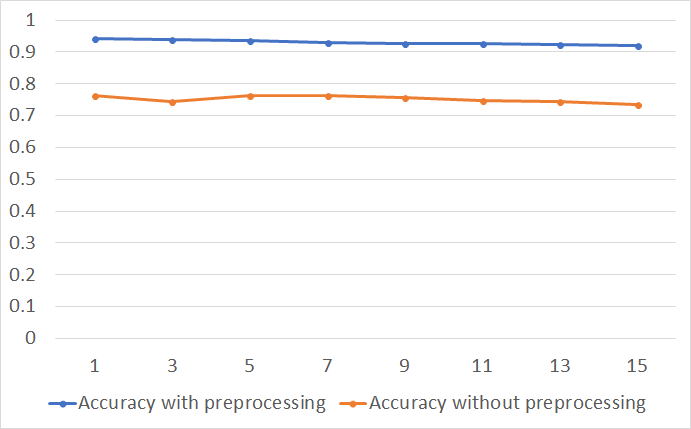
\includegraphics[width=.8\textwidth]{fig//KNN_K}
	\caption{KNN performance under different values of $k$.}\label{fig:KNN_K}
\end{figure}


In our experiment, we enumerate different values of $k$ from $1$ to $15$, and for each such value, we find the optimal PCA ratio on the validation set. We then test the KNN performance for different $k$ values on the test set, with their optimized PCA ratios. The experiment results are shown in Figure~\ref{fig:KNN_K}. Kind of surprisingly, the performance of KNN seems not to vary much with $k$, both with and without preprocessing. One interpretation of this phenomenon is that we have thousands of training samples for each category (i.e., hand-writing digit), and varying the value of $k$ over such a small range merely hurts the outcome of the majority voting among the neighbors of a testing sample. 


\subsubsection{Performance under Optimal Parameters}
In this part, we feed all the training samples (instead of only 10000 samples as in the previous experiments) into the model, and use all the test data in the testing phase. For KNN with preprocessing, the optimal parameter settings with PCA ratio equal to $0.8$ and $k=1$ lead to the accuracy of $98.40\%$. For KNN without preprocessing, the accuracy $88.12\%$ is achieved at PCA raio equal to $0.6$ and $k=5$. As we can see, since KNN is sensitive to spatial shifting, our preprocessing steps significantly improve the performance of KNN. The detailed performance of KNN on each category is shown in Table\ref{tbl:KNN_with_score}.

\begin{table}[!htb]
	\centering
	\small 
	\caption{KNN performance with / without preprocessing}
		%\centering
		\begin{tabular}{ccccc}
			& precision & recall & f1-score & support \\
			0     & 1     & 0.99  & 0.99  & 992 \\
			1     & 0.99  & 0.99  & 0.99  & 1193 \\
			2     & 0.98  & 0.99  & 0.99  & 1031 \\
			3     & 0.98  & 0.97  & 0.98  & 1030 \\
			4     & 0.98  & 0.99  & 0.98  & 927 \\
			5     & 0.99  & 0.98  & 0.98  & 894 \\
			6     & 0.99  & 0.99  & 0.99  & 1021 \\
			7     & 0.98  & 0.99  & 0.98  & 1028 \\
			8     & 0.98  & 0.98  & 0.98  & 922 \\
			9     & 0.98  & 0.96  & 0.97  & 962 \\
			avg / total & 0.98  & 0.98  & 0.98  & 10000 \\
		\end{tabular}%
		%\hspace{.01in}
		%\centering
		%\caption{}
		\begin{tabular}{ccccc}
			& precision & recall & f1-score & support \\
			0     & 0.92  & 0.96  & 0.94  & 992 \\
			1     & 0.87  & 0.99  & 0.93  & 1193 \\
			2     & 0.94  & 0.88  & 0.91  & 1031 \\
			3     & 0.86  & 0.86  & 0.86  & 1030 \\
			4     & 0.87  & 0.84  & 0.85  & 927 \\
			5     & 0.88  & 0.84  & 0.86  & 894 \\
			6     & 0.93  & 0.94  & 0.93  & 1021 \\
			7     & 0.88  & 0.88  & 0.88  & 1028 \\
			8     & 0.89  & 0.79  & 0.84  & 922 \\
			9     & 0.77  & 0.81  & 0.79  & 962 \\
			avg / total & 0.88  & 0.88  & 0.88  & 10000 \\
		\end{tabular}%
	\label{tbl:KNN_with_score}%
\end{table}%

\subsection{Support Vector Machine}
In this part, we perform Support Vector Machine, or SVM, on the given data set as well as our processed data set. We choose this algorithm because it is generally expressive (with the use of a kernel), robust, and also widely applied in many real world problems before the outbreak of deep learning. It is reasonable to regard a finely tuned SVM as the best-performed representative of traditional classification models. By comparing the performance of SVM and neural networks, we can discuss the pros and cons between the traditional classifiers and the deep learning models.

In our experiment, we also randomly select 30\% of the training samples as the validation set, and employ hold-out validation to optimize the parameter settings before applying our model to the test set. 

Each image in the MNIST data set is $45\times 45$ dimensional. Although this is almost the simplest image data set we can find, we still do not expect the samples to be trivially linear separable. Therefore, throughout our experiment, we use the radial basis function kernel, or simply rbf kernel for SVM. The rbf kernel on two samples $x$ and $x'$ is defined as $K(x,x') = \exp(- \gamma \left\|x-x' \right\|)^2$, where $\gamma = \frac{1}{2\sigma^2}$ and $\sigma$ is a free parameter. The rbf kernel can be interpreted as a similarity measure. Compared with the linear kernel, the rbf kernel is richer in expressiveness, and can handle the case where data points are not linearly separable. The drawback of rbf kernel is that it is very sensible to the specific values of the parameters. To ensure a better performance, we need to rely on cross validation to find the proper parametric settings, which can be quite time consuming. On the contrary, the linear kernel features fewer parameters and less time cost, and is generally well-performed on various problems. The disadvantage is that the linear kernel is basically limited to situations where the data samples are linearly separable. Since the linear kernel can be regarded as a special case of the rbf kernel, we can anticipate the rbf kernel to achieve better performance with finely tuned parameters. Since we want SVM to represent the best performance of traditional models in our experiments, the rbf kernel is a natural choice. 


\begin{table}[!htb]
	\centering
	\small 
	\caption{SVM performance with / without preprocessing}
	%\centering
		\begin{tabular}{ccccc}
			& precision & recall & f1-score & support \\
			0     & 0.99  & 0.99  & 0.99  & 992 \\
			1     & 0.99  & 0.99  & 0.99  & 1193 \\
			2     & 0.99  & 0.99  & 0.99  & 1031 \\
			3     & 0.99  & 0.98  & 0.99  & 1030 \\
			4     & 0.98  & 0.99  & 0.99  & 927 \\
			5     & 0.99  & 0.98  & 0.99  & 894 \\
			6     & 0.99  & 0.99  & 0.99  & 1021 \\
			7     & 0.98  & 0.99  & 0.98  & 1028 \\
			8     & 0.98  & 0.99  & 0.99  & 922 \\
			9     & 0.98  & 0.97  & 0.98  & 962 \\
			avg / total & 0.99  & 0.99  & 0.99  & 10000 \\
		\end{tabular}%
	%\hspace{.01in}
	%\centering
	%\caption{}
		\begin{tabular}{ccccc}
			& precision & recall & f1-score & support \\
			0     & 0.93  & 0.97  & 0.95  & 992 \\
			1     & 0.97  & 0.96  & 0.97  & 1193 \\
			2     & 0.92  & 0.93  & 0.93  & 1031 \\
			3     & 0.93  & 0.92  & 0.93  & 1030 \\
			4     & 0.94  & 0.92  & 0.93  & 927 \\
			5     & 0.93  & 0.91  & 0.92  & 894 \\
			6     & 0.96  & 0.96  & 0.96  & 1021 \\
			7     & 0.94  & 0.92  & 0.93  & 1028 \\
			8     & 0.9   & 0.9   & 0.9   & 922 \\
			9     & 0.88  & 0.9   & 0.89  & 962 \\
			avg / total & 0.93  & 0.93  & 0.93  & 10000 \\
		\end{tabular}%
	
	\label{tbl:SVM_with_score}%
\end{table}%

The sklearn.svm module provides the SVC class that implements the basic functions of SVM. Two crucial parameters of this class include the error term penalty parameter $C$, and the rbf kernel coefficient $\gamma$. We refer to cross validation to optimize the parameter settings. We also enumerate various PCA ratios and keep the ratio of highest accuracy from the validation set. We will not go through the detailed procedure of testing the influence of various parameters in this report, since they are already covered in our third homework. Our codes for SVM are in files \texttt{SVM.py} and \texttt{SVM\_without\_preprocessing.py}. In the following, we simply list the SVM performance on the test set. The accuracy with preprocessing is $98.75\%$, which is achieved at PCA ratio equal to $0.85$, $C=5$ and $\gamma = 5 \times 10^{-7}$. The accuracy of SVM without preprocessing of the data set is $93.22\%$, which is achieved at PCA ratio equal to $0.65$, $C=6$ and $\gamma = 10^{-6}$. The detailed performance of KNN on each category is shown in Table~\ref{tbl:SVM_with_score}.

\subsection{Ensemble Methods}
In this part, we try ensemble methods on our given problem. Typical ensemble methods include bagging methods, random forests, AdaBoosting, Gradient Tree Boosting, etc, and the scikit-learn library has provided most of these methods. The principle of parallel ensemble methods like bagging methods is to build several independent classifiers and average their predictions. Since the variance is reduced, the combined classifier is expected to perform better than any of the individual base classifier. By contrast, the sequential ensemble methods like boosting combine base classifiers sequentially and tries to reduce the bias of the combined classifier.

In our experiment, we only implement a simple voting classifier, by combining the predictions of our previous KNN and SVM classifiers. We use soft voting by requiring every base classifier to report a probability of assigning the sample to each category, and the final prediction is the category with highest average probability. The parameters for KNN and SVM are cross-validated, and our implementation codes are in file \texttt{voting.py}. The accuracy of the voting classifier on the test set is $98.40\%$, which is achieved at PCA ratio equal to $0.8$, $k=1$, $C=6$ and $\gamma = 10^{-6}$. The detailed performance on each category is shown in Table\ref{tbl:voting}.

\begin{table}[!htb]
	\centering
	\small 
	\caption{Voting performance with preprocessing.}
	\begin{tabular}{ccccc}
		& precision & recall & f1-score & support \\
		0     & 1     & 0.99  & 0.99  & 992 \\
		1     & 0.99  & 0.99  & 0.99  & 1193 \\
		2     & 0.98  & 0.99  & 0.99  & 1031 \\
		3     & 0.98  & 0.97  & 0.98  & 1030 \\
		4     & 0.98  & 0.99  & 0.98  & 927 \\
		5     & 0.99  & 0.98  & 0.98  & 894 \\
		6     & 0.99  & 0.99  & 0.99  & 1021 \\
		7     & 0.98  & 0.99  & 0.98  & 1028 \\
		8     & 0.98  & 0.98  & 0.98  & 922 \\
		9     & 0.98  & 0.96  & 0.97  & 962 \\
		avg / total & 0.98  & 0.98  & 0.98  & 10000 \\
	\end{tabular}%
	\label{tbl:voting}%
\end{table}%


Surprisingly, the combined performance of the two classifiers is actually worse than using the SVM classifier itself. One possible reason is we did not finely tune the parameter values since the grid searching of so many parameters is quite time consuming. Another reason is our voting classifier is composed of only two base classifiers, but in common practice the ensemble classifier may consist of more than a hundred base classifiers to reduce the variance. In addition, the base classifiers of an ensemble model should generally be independent of each other---they should be built on different subsets of the training data, or built upon different combinations of features. Only when the base classifiers are independent can the variance of the ensemble be truly reduced. Another reason is that the performance of our two previous models are already good enough, and it is difficult to reduce the variance simply by averaging the two classifiers. More discussion about the comparison between an ensemble model and each individual model can be found in~\cite{dvzeroski2004combining}. 

The lesson we can learn from this experiment is that a simple combination of several classifiers does not guarantee better performance. We need to further check whether the base classifiers are independent of each other, and whether the parallel ensemble model can indeed reduce the variance and help avoid the noise in the data set.

\section{Capsule Networks}
In this section, we learn the Capsule Networks proposed by Hinton et al.\ and apply it to our given data set. The Capsule Network was first introduced back in 2011\cite{hinton2011transforming}, where Hinton el al.\ pointed out many of the key features of a capsule, but they did not find a way to train the Capsule Networks at that time. Until very recently, in 2017, they claimed to find a way to make the whole architecture work and the Capsule Network achieves state-of-the-art performance on the MNIST data set\cite{sabour2017dynamic}. 

In this project, we studied the intuition, architecture and the routing algorithm of the Capsule Networks, and try to reproduce the results on our given data set. We list our understanding of the related papers as well as the experiment results on our given problem as follows.

\subsection{Intuition behind the Capsule Network}
Research about the neuroscience tells us that humans learn and analyze visual information hierarchically. When we look at an image of a person, our brain recognizes two eyes, one nose, and one mouth, and putting the lower-level features together, we learn that there is a person in the image. This is the original intuition of Convolutional Neural Networks---they recognize lower-level features from earlier layers in the network, and pass the features to later layers where high-level features are extracted. 

\begin{figure}[!htb]
	\centering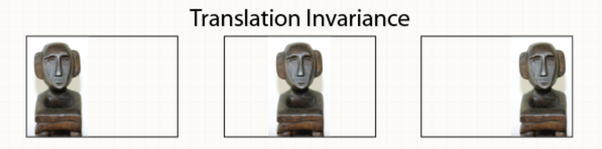
\includegraphics[width=1.0\textwidth]{fig//invariance}
	\caption{Translational invariance guarantees CNN will recognize the three items as the same, since position does not matter to CNN.\protect\footnotemark }\label{fig:invariance}
\end{figure}

\footnotetext{Image source: https://www.quora.com/What-is-the-difference-between-equivariance-and-invariance-in-Convolution-neural-networks.}

Convolutional Neural Networks benefit from a key property called translational invariance. This property basically states that the position of the item in the image does not affect how CNN classifies the item, as illustrated in Figure~\ref{fig:invariance}. The internal representation of the network will be roughly the same if a pattern is translated across the image. The way that CNN achieves translational invariance is to use the same kernel all over the image to detect the occurrence of the same feature in multiple locations. This trick also makes the system run faster due to the reduction in parameters through sharing them over all locations in the image.

\begin{figure}[!htb]
	\centering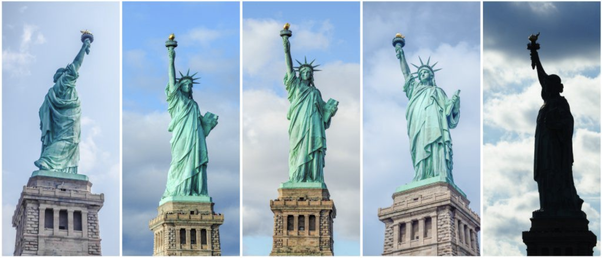
\includegraphics[width=\textwidth]{fig//equivariance}
	\caption{Illustration of the equivariance property.\protect\footnotemark }\label{fig:equivariance}
\end{figure}

\footnotetext{Image source: https://www.quora.com/What-is-the-difference-between-equivariance-and-invariance-in-Convolution-neural-networks.}

Convolutional Neural Networks, however, cannot achieve the equivariance property. The concept of equivariance is similar to invariance, but in addition to having the classification irrelevant to the position, equivariance also asks to predict where the object is. As an example, in Figure~\ref{fig:equivariance}, our brain would correctly identify that these are all the statue of liberty, regardless of the different angles and lighting conditions. CNN is unable to disentangle transformations to the image, such as rotation, changes in color, or lighting conditions, and it will perform terribly on the example of Figure~\ref{fig:equivariance} unless explicitly trained for these angles.

\begin{figure}[!htb]
	\centering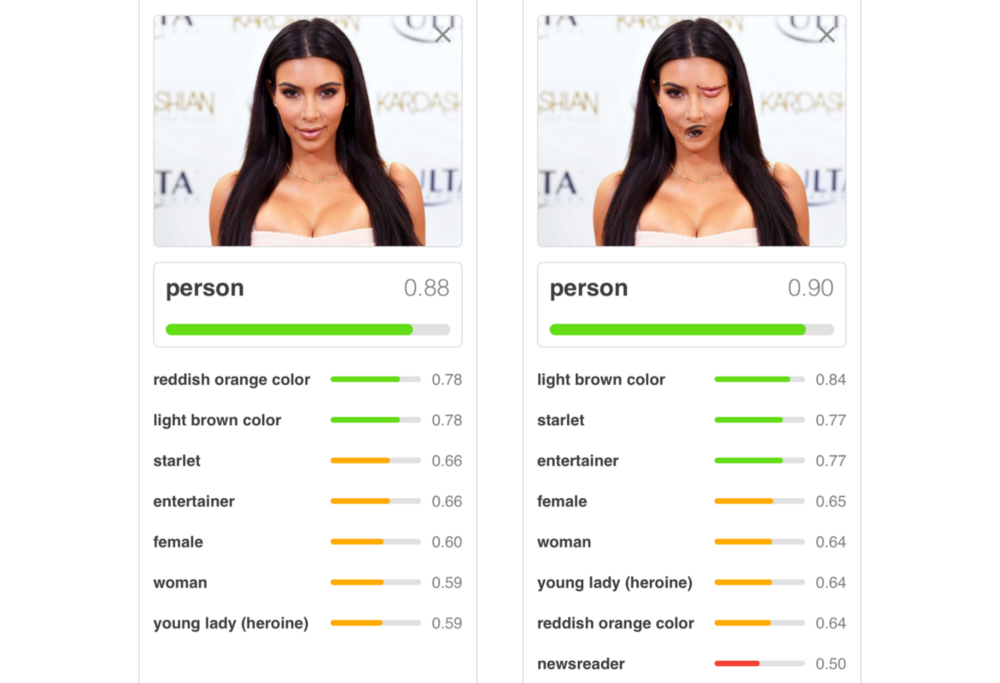
\includegraphics[width=\textwidth]{fig//maxpooling}
	\caption{CNN classifies both images as human faces because of overly lenient translational invariance.\protect\footnotemark }\label{fig:maxpooling}
\end{figure}

\footnotetext{Image source: https://hackernoon.com/capsule-networks-are-shaking-up-ai-heres-how-to-use-them-c233a0971952.}

This problem can be credited to Max Pooling. When Kunihiko Fukushima first applied Max Pooling to his Neocognitron network\cite{fukushima1983neocognitron} to allow translational invariance, it was good because the initial idea of Max Pooling makes sense in his digit recognizing problem. However, this is not the case in modern deep learning problems, since we want to detect all parts that make up the whole, and we also need all these elements to be spatially related to each other. Max Pooling is just too lenient with translational invariance, in that it only conveys very vague description about spatial information from layer to layer. For example in Figure~\ref{fig:maxpooling}, CNN would classify both images as human faces despite that the locations of the mouth and the eye have been exchanged, because CNN detects all the necessary lower-level features and Max Pooling collects these lower-level features with minor concern of their spatial translations. 

\begin{figure}[!htb]
	\centering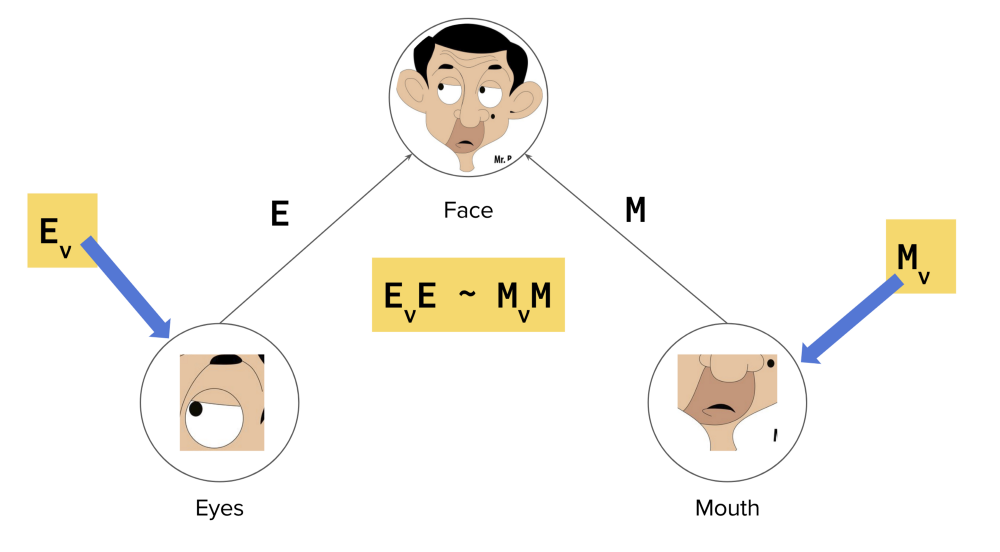
\includegraphics[width=.8\textwidth]{fig//partwhole}
	\caption{The pose matrices associate the parts with the whole.\protect\footnotemark }\label{fig:partwhole}
\end{figure}

\footnotetext{Image source: https://hackernoon.com/uncovering-the-intuition-behind-capsule-networks-and-inverse-graphics-part-i-7412d121798d.}

\begin{figure}[!htb]
	\centering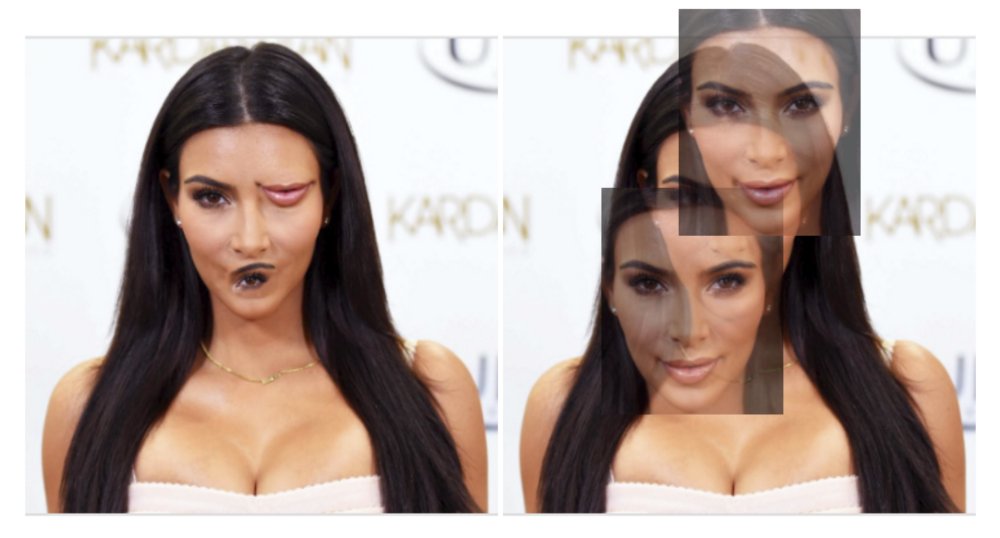
\includegraphics[width=.8\textwidth]{fig//agreement}
	\caption{The estimations based on the eye and the mouth do not match.\protect\footnotemark }\label{fig:agreement}
\end{figure}

\footnotetext{Image source: https://hackernoon.com/uncovering-the-intuition-behind-capsule-networks-and-inverse-graphics-part-i-7412d121798d.}

Hinton argues that in order to correctly do classification and object recognition, it is important to preserve hierarchical pose relationships between object parts. Given the location of a mouth, humans can directly estimate where the face might be regardless of the variation of the viewpoint. There exists a pose matrix that represents the relationship between the parts and the whole, as illustrated in Figure~\ref{fig:partwhole}. When these relationships are built into internal representation of data, it becomes very easy for a model to understand that the thing that it sees is just another view of something that it has seen before. This solves the problem in Figure~\ref{fig:equivariance} about how to interpret the Statue of Liberty from different viewpoints as the same thing. Furthermore, given an image like in Figure~\ref{fig:agreement}, the model will estimates the positions of the face from both the eye and the mouth, and based on these part-whole relationships the model quickly finds out the two estimations do not match with each other. In this case, the model with these built-in relationships will not classify the image as a face, even though it contains all the necessary features that make up a face.  

\subsection{Dynamic Routing with Capsules}
Unlike CNNs, capsules encode the probability of a feature as the length of the output vector, and the state of the detected feature is encoded as the direction in which that vector points to. Therefore, when the feature moves around in the image, the output vector length stays the same, denoting the probability of this feature does not change, but the orientation of the output vector does change. 

\begin{figure}[!htb]
	\centering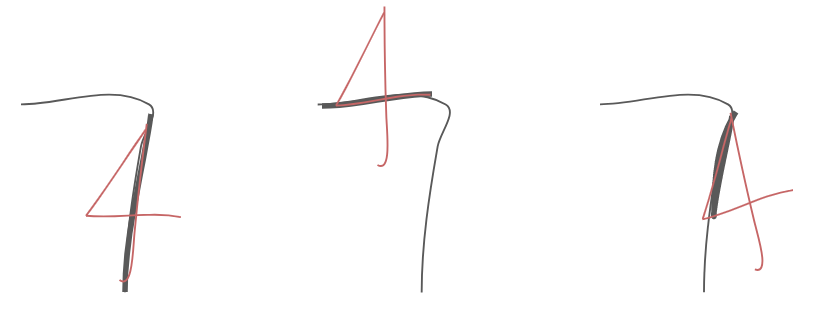
\includegraphics[width=.8\textwidth]{fig//routing}
	\caption{From lower level capsules to higher level ones.}\label{fig:routing}
\end{figure}

When receiving vectors from lower level capsules, the higher level capsule first generates the higher level feature by making estimations based on each individual input vector. These vectors are then multiplied by the corresponding weight matrices $W$ that encode spatial and perhaps other relationships between lower level features and higher level feature. Consider the example in Figure~\ref{fig:routing}. Suppose the bold lines denote the low-level features detected from the input image, a vertical line, a horizontal line, and a short diagonal line, which together make up the digit $7$. The high level capsule for digit $4$ receives these input vectors, and multiply them with their corresponding matrices to generate the possible positions and rotations of digit $4$. Clearly, the positions of the three individual estimations do not agree with each other, and hence the probability for a digit $4$ is low. On the contrary, the estimations of digit $7$ are quite consistent across the low-level features, and the probability of digit $7$ is much higher. 



\bibliographystyle{ieee}
\bibliography{egbib}
\end{document}
